\section{本研究で用いるプレイヤ}
\subsection{Nタプルネットワーク}
\label{sec:Ntuple}

% 2048における最も成功したプレイヤの多くは,Nタプルネットワークに基づく評価関数を強化学習によってチューニングするアプローチを採用している~\cite{SzJa14}.
% Gueiらの最新のプレイヤ~\cite{GuCW22}も,Matsuzaki~\cite{Mats16}が提案したタプルの組合せをベースに,Expectimax探索やMultistaging\cite{YWHC16},Optimistic Initialization,Tile Downgrading\cite{GuCW22}などの改良を加えることで高い性能を達成している.

本研究では,表\ref{tuples}に示すとおり,1タプルから9タプルまでのNタプルネットワークを合計で15種類設計して用いた.

まず,特徴抽出する $N$ マス(図では丸で示される)がすべて上下左右に連結しているようなものを,有効な $N$ タプルとした.
その結果,$N=1$ から $N=9$ まで順に有効な $N$ タプルが,3通り,2通り,5通り,6通り,9通り,8通り,7通り,3通り,1通り得られた.
指定した大きさ $N$ について,有効な $N$ タプルをすべて含むNタプルネットワークを $N$-Full と名付けた(本文および図表においては,より短く \textsf{1F} などと表記する).

2048におけるNタプルネットワークの設計では,有望そうな形をいくつか人手で作成し,それを平行移動させて得られる
タプルを組合せる手法がよく用いられている~\cite{SzJa14,YWHC16,Jask17}.
そこで,この考え方に基づくタプルの組合せを $N$-Manual として設計した(本文および図表においては,より短く \textsf{3M} などと表記する).
ただし,1タプル,2タプル,9タプルでは,有効な $N$ タプルがすべて有望そうな形をしていることから,\textsf{1M},\textsf{2M},\textsf{9M}はそれぞれ\textsf{1F},\textsf{2F},\textsf{9F}と同一である.

なお,Nタプルネットワークで評価値を計算する際には,ミニ2048の盤面の持つ対称性(回転・反転)を活用し,各タプルに対して8通りの位置からのサンプリングを行う.また,後述する Multistaging により各プレイヤはNタプルネットワークを2つ持つことから,表\ref{tuples}に示すパラメータ数は,タプルサイズを $N$ として
\[
 \mbox{パラメータ数} = 11^N \times 2
\]
により計算される値である.

\begin{table}[t]
  \caption{タプルサイズと組合せの一覧}
  \label{tuples}
  \centering\begin{tabular}{llr}
   \hline
   \hline
   名称 & \hspace{20pt}タプルの組合せ & パラメータ数\\
   \hline
   \raisebox{10pt}{\textsf{1F}}\raisebox{28pt}{~}
          & 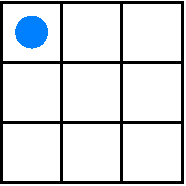
\includegraphics[height=22pt]{pdf/tuples/1tuple_6_page1.pdf}~
            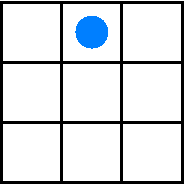
\includegraphics[height=22pt]{pdf/tuples/1tuple_6_page2.pdf}~
            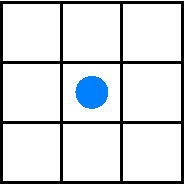
\includegraphics[height=22pt]{pdf/tuples/1tuple_6_page3.pdf} & \raisebox{10pt}{66}\\
   \hline
   \raisebox{10pt}{\textsf{2F}}\raisebox{28pt}{~}
          & 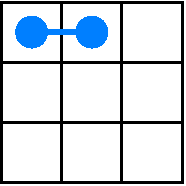
\includegraphics[height=22pt]{pdf/tuples/2tuple_12_page1.pdf}~
            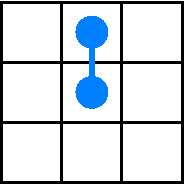
\includegraphics[height=22pt]{pdf/tuples/2tuple_12_page2.pdf}& \raisebox{10pt}{484}\\
   \hline
   \raisebox{10pt}{\textsf{3M}}\raisebox{28pt}{~}
          & 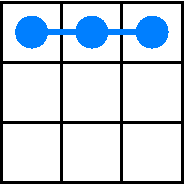
\includegraphics[height=22pt]{pdf/tuples/3tuple_144_page1.pdf}~
            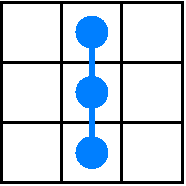
\includegraphics[height=22pt]{pdf/tuples/3tuple_144_page3.pdf}~
            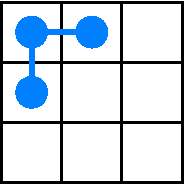
\includegraphics[height=22pt]{pdf/tuples/3tuple_144_page2.pdf}& \raisebox{10pt}{7,986}\\
   \hline
   \raisebox{10pt}{\textsf{3F}}\raisebox{28pt}{~}
          & 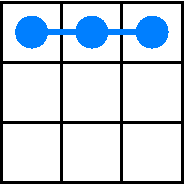
\includegraphics[height=22pt]{pdf/tuples/3tuple_2673_page1.pdf}~
            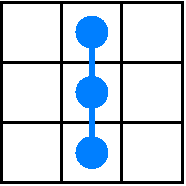
\includegraphics[height=22pt]{pdf/tuples/3tuple_2673_page5.pdf}~
            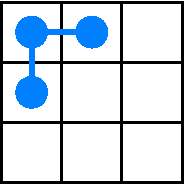
\includegraphics[height=22pt]{pdf/tuples/3tuple_2673_page2.pdf}~
            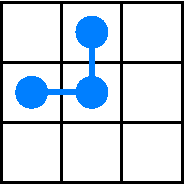
\includegraphics[height=22pt]{pdf/tuples/3tuple_2673_page4.pdf}~
            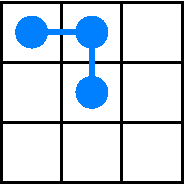
\includegraphics[height=22pt]{pdf/tuples/3tuple_2673_page3.pdf}& \raisebox{10pt}{13,310}\\
   \hline
   \raisebox{10pt}{\textsf{4M}}\raisebox{28pt}{~}
          & 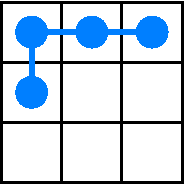
\includegraphics[height=22pt]{pdf/tuples/4tuple_301_page1.pdf}~
            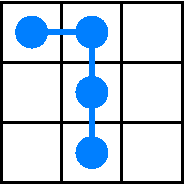
\includegraphics[height=22pt]{pdf/tuples/4tuple_301_page3.pdf}~
            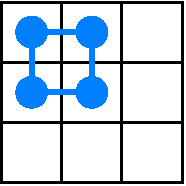
\includegraphics[height=22pt]{pdf/tuples/4tuple_301_page2.pdf}& \raisebox{10pt}{87,846}\\
   \hline
   % \raisebox{10pt}{\textsf{4F}}\raisebox{28pt}{~}
   \multirow{2}{*}{\textsf{4F}}\raisebox{28pt}{~}
          & 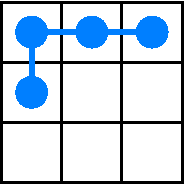
\includegraphics[height=22pt]{pdf/tuples/4tuple_44755_page1.pdf}~
            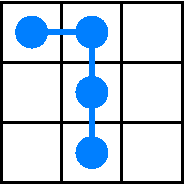
\includegraphics[height=22pt]{pdf/tuples/4tuple_44755_page5.pdf}~
            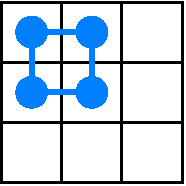
\includegraphics[height=22pt]{pdf/tuples/4tuple_44755_page3.pdf}& \multirow{2}{*}{175,692}\\
          & 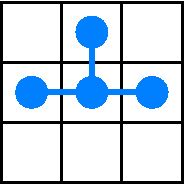
\includegraphics[height=22pt]{pdf/tuples/4tuple_44755_page6.pdf}~
            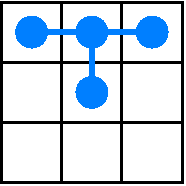
\includegraphics[height=22pt]{pdf/tuples/4tuple_44755_page2.pdf}~
            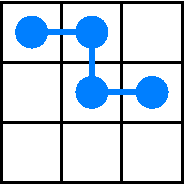
\includegraphics[height=22pt]{pdf/tuples/4tuple_44755_page4.pdf}\\
   \hline
   \raisebox{10pt}{\textsf{5M}}\raisebox{28pt}{~}
          & 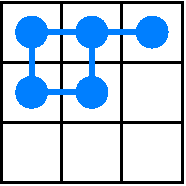
\includegraphics[height=22pt]{pdf/tuples/5tuple_298_page1.pdf}~
            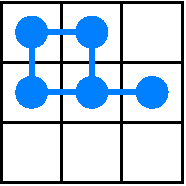
\includegraphics[height=22pt]{pdf/tuples/5tuple_298_page2.pdf}~
            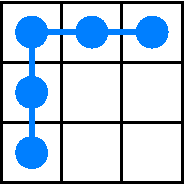
\includegraphics[height=22pt]{pdf/tuples/5tuple_298_page3.pdf} & \raisebox{10pt}{966,306}\\
   \hline
   \multirow{2}{*}{\textsf{5F}}\raisebox{28pt}{~}
          & 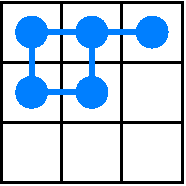
\includegraphics[height=22pt]{pdf/tuples/5tuple_896673_page1.pdf}~
            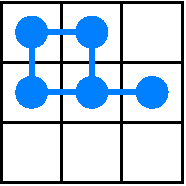
\includegraphics[height=22pt]{pdf/tuples/5tuple_896673_page3.pdf}~
            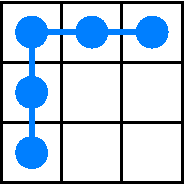
\includegraphics[height=22pt]{pdf/tuples/5tuple_896673_page4.pdf}~
            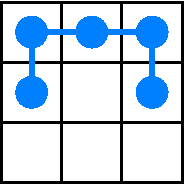
\includegraphics[height=22pt]{pdf/tuples/5tuple_896673_page2.pdf}~
            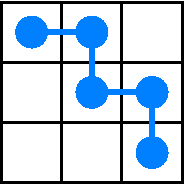
\includegraphics[height=22pt]{pdf/tuples/5tuple_896673_page5.pdf}& \multirow{2}{*}{2,898,918}\\
          & 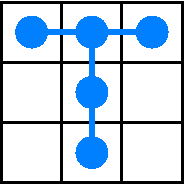
\includegraphics[height=22pt]{pdf/tuples/5tuple_896673_page6.pdf}~
            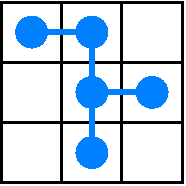
\includegraphics[height=22pt]{pdf/tuples/5tuple_896673_page7.pdf}~
            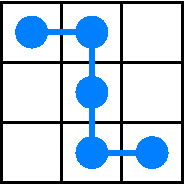
\includegraphics[height=22pt]{pdf/tuples/5tuple_896673_page8.pdf}~
            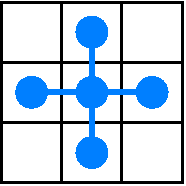
\includegraphics[height=22pt]{pdf/tuples/5tuple_896673_page9.pdf}\\
   \hline
   \raisebox{10pt}{\textsf{6M}}\raisebox{28pt}{~}
          & 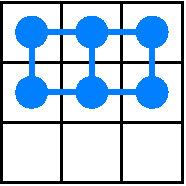
\includegraphics[height=22pt]{pdf/tuples/6tuple_16_page1.pdf}~
            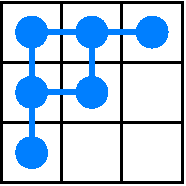
\includegraphics[height=22pt]{pdf/tuples/6tuple_16_page2.pdf} & \raisebox{10pt}{7,086,244}\\
   \hline
   \multirow{2}{*}{\textsf{6F}}\raisebox{28pt}{~}
          & 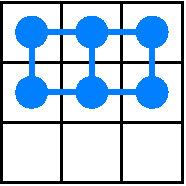
\includegraphics[height=22pt]{pdf/tuples/6tuple_26835_page1.pdf}~
            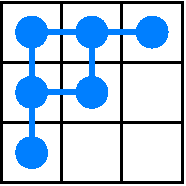
\includegraphics[height=22pt]{pdf/tuples/6tuple_26835_page2.pdf}~
            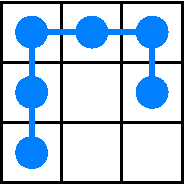
\includegraphics[height=22pt]{pdf/tuples/6tuple_26835_page3.pdf}~
            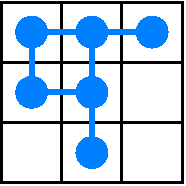
\includegraphics[height=22pt]{pdf/tuples/6tuple_26835_page4.pdf}& \multirow{2}{*}{28,344,976}\\
          & 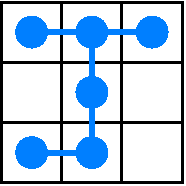
\includegraphics[height=22pt]{pdf/tuples/6tuple_26835_page5.pdf}~
            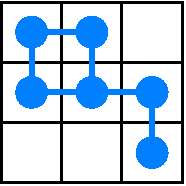
\includegraphics[height=22pt]{pdf/tuples/6tuple_26835_page6.pdf}~
            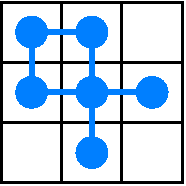
\includegraphics[height=22pt]{pdf/tuples/6tuple_26835_page7.pdf}~
            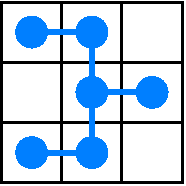
\includegraphics[height=22pt]{pdf/tuples/6tuple_26835_page8.pdf}\\
   \hline
   \raisebox{10pt}{\textsf{7M}}\raisebox{28pt}{~}
          & 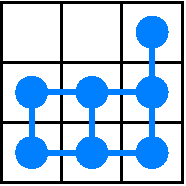
\includegraphics[height=22pt]{pdf/tuples/7tuple_0_page1.pdf} & \raisebox{10pt}{38,974,342}\\
   \hline
   \raisebox{10pt}{\textsf{7F}}\raisebox{28pt}{~}
          & 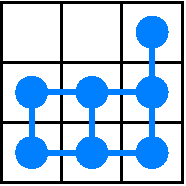
\includegraphics[height=22pt]{pdf/tuples/7tuple_248_page1.pdf}~
            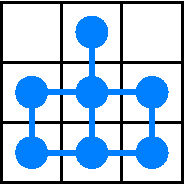
\includegraphics[height=22pt]{pdf/tuples/7tuple_248_page2.pdf}~
            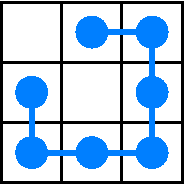
\includegraphics[height=22pt]{pdf/tuples/7tuple_248_page3.pdf}~
            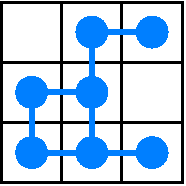
\includegraphics[height=22pt]{pdf/tuples/7tuple_248_page4.pdf}& \multirow{2}{*}{272,820,394}\\
          & 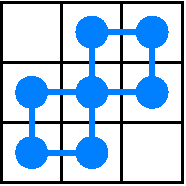
\includegraphics[height=22pt]{pdf/tuples/7tuple_248_page5.pdf}~
            \includegraphics[height=22pt]{pdf/tuples/7tuple_248_page6.pdf}~
            \includegraphics[height=22pt]{pdf/tuples/7tuple_248_page7.pdf}\\
   \hline
   \raisebox{10pt}{\textsf{8M}}\raisebox{28pt}{~}
          & \includegraphics[height=22pt]{pdf/tuples/8tuple_0_page1.pdf} & \raisebox{10pt}{428,717,762}\\
   \hline
   \raisebox{10pt}{\textsf{8F}}\raisebox{28pt}{~}
          & \includegraphics[height=22pt]{pdf/tuples/8tuple_6_page1.pdf}~
            \includegraphics[height=22pt]{pdf/tuples/8tuple_6_page2.pdf}~
            \includegraphics[height=22pt]{pdf/tuples/8tuple_6_page3.pdf} & \raisebox{10pt}{1,286,153,286}\\
   \hline
   \raisebox{10pt}{\textsf{9F}}\raisebox{28pt}{~}
          & \includegraphics[height=22pt]{pdf/tuples/9tuple_0_page1.pdf} & \raisebox{10pt}{4,715,895,382}\\
   \hline
  \end{tabular}
\end{table}

\subsection{Nタプルネットワークの学習方法}

Nタプルネットワークの重みは,afterstate 間の評価値の差に基づくTD学習法の改良手法によって調整した.
本研究で用いるNタプルネットワークの学習では,以下の技術を用いた.
\begin{description}
  % \item [対称性サンプリング] 各タプルについて,鏡面,回転対称用いてを1つの盤面から,8つの対称位置からサンプリングする. これにより,少ないタプル数で盤面全体から特徴を抽出することができる.
  \item [Multistaging] ゲームの進行に応じて重みを参照するテーブルを切り替える.本研究では,2ステージとし,512 のタイルができる前後でステージを分けた.
  \item [Temporal coherence 学習(TC学習)] TC学習は学習率自動調整機能を備えたTD学習で,Ja\'{s}kowski~\cite{Jask17}が始めて2048に導入した.TC学習では,更新しようとする重みごとに,それまでの学習ステップの更新量の総和を,更新量の絶対値の総和で割った値を学習率とする.本研究の実装では,次の Optimistic initialization の効果がある程度残るように,学習率の最大を 0.5 でクリッピングする変更を加えた.
  \item [Optimistic initialization] 学習段階での探索を広く行うために,重みを(ゼロではなく)大きな値で初期化する.本研究で用いたNタプルの学習では,すべての afterstate の初期値を $\mathit{OI}=0$,$\mathit{OI}=1200$,$\mathit{OI}=5400$ の3通りとした.
\end{description}

それぞれのNタプルニューラルネットワークに対して,$5\times 10^8$ 局面分のデータで学習を行った.著者らの先行研究~\cite{TeKM23}において,この学習量は学習が収束するのに十分であった.

\subsection{Nタプルネットワークを評価関数とするプレイヤ}

本研究で用いるプレイヤは,前節の方法で重みを調整したNタプルネットワークを評価関数とし,Expectimax探索により手を選択する.
Expectimax探索の実装については,著者らの先行研究~\cite{Terauchi24} で用いたものをそのまま利用した.

以上より本研究で用いる各プレイヤは,Nタプルネットワークの組合せ(\textsf{1F}, \textsf{2F}, \ldots, \textsf{9F}, \textsf{3M}, \ldots, \textsf{8M}),学習における Optimistic initialization の初期値($\mathit{OI}\in \{0, 1200, 5400\}$),探索の深さ(Greedy,$d\in \{2, 3, \ldots, 6\}$) の3つにより決定される.(先読みが1手の場合は,慣習に従い Greedy と表記する.)

% \newpage
% \section{Expectimax探索}
% \label{sec:expectimax}
% Expectimax探索は,確率的一人ゲームにおける標準的な探索手法である.
% ミニ2048のゲームの進行は,state におけるプレイヤの選択と,afterstate における新規タイルの出現が交互に起こる.
% したがって,ミニ2048のゲーム木は,根が現在の state に対応し,根から葉への各パス上に,afterstate に対応するノード(chance ノード)と state に対応するノード(max ノード)が交互に現れる.本研究では,ミニ2048のゲーム木の高さ(探索の深さ)を,各パス上の afterstate に対応するノードの数と定める.例えば,高さ2 のミニ2048のゲーム木は,根,afterstate に対応するノードの層,state に対応するノードの層,afterstate に対応するノードの層,の合計4層からなる(図~\ref{result.Expectimax}).

% Expectimax探索では,ゲーム木の各ノードに対して次のように再帰的に計算を行う.
% \begin{itemize}
%  \item maxノードでは,子要素の値のうちの最大値を計算する.
%  \item chanceノードでは,子要素の値を,その出現確率を用いた重み付き平均を計算する.
% \end{itemize}
% Expectimax探索プレイヤは,Expectimax探索によって得られた子ノードのうち,評価値の最も大きなものを選択する.

% 図\ref{result.Expectimax}に深さ2のExpectimax探索の例を示す.

% \begin{figure}[t]
%   \centering
%   \includegraphics[width=.99\linewidth]{pdf/expectimax.pdf}
%   \caption{深さ 2 のExpectimax 探索の例}
%   \label{result.Expectimax} 
% \end{figure}

% ミニ2048のゲーム木では,特に,同じ afterstate が複数出現する.
% そのような同じ afterstate をまとめる(合流)工夫を実装した.ただし,合流を考慮しない Expectimax と結果が一致するよう,同じ afterstate であってもゲーム木中の深さが異なる場合には別のものとして扱った.この工夫により,特に深い探索において大幅な高速化が実現された.
% 本研究では\cite{Terauchi24}で実装したExpectimax探索を用いた.
% \newpage